\documentclass{beamer}
%%%%%% UNOFFICIAL ICL BEAMER TEMPLATE V.0.1 %%%%%%
% This is a basic LaTeX Beamer template that I customised to have the logo of ICL and a background picture. Mind that this is NOT an official ICL template but it may still be useful for informal presentations.
% The official ICL graphical identity resources can be found here: http://www3.imperial.ac.uk/graphicidentity
% Please drop me an e-mail or comment via Twitter @AJunyentFerre if you found this was useful or have any suggestion to improve it.
%%%%%%

\usepackage[english]{babel}
\usepackage{xcolor}
\usepackage{xmpmulti}
\usepackage{amsmath}
\usepackage{dsfont}
\usepackage{tikz}
\usepackage{eucal}
\usetikzlibrary{positioning,angles,quotes}
\usepackage{url}
\usepackage{graphicx}
\usepackage{cmbright}
\usepackage{framed}


\usetikzlibrary{pgfplots.groupplots,arrows.meta,shadows,positioning,angles,quotes}
%usetikzlibrary{matrix,chains,positioning,decorations.pathreplacing,arrows}
\usetikzlibrary{shapes.geometric}
\usetikzlibrary{positioning}
\usepackage{pgfplots}

\DeclareMathOperator*{\argmax}{arg\,max}

\definecolor{Maroon}{cmyk}{0, 0.87, 0.68, 0.32}
\definecolor{RoyalBlue}{cmyk}{1, 0.50, 0, 0}
\definecolor{skymagenta}{rgb}{0.81, 0.44, 0.69}

\newenvironment{takeaway}[1]{%
\definecolor{shadecolor}{gray}{0.9}%
	\begin{shaded}{\color{skymagenta}\noindent\textsc{#1}}\\%
	}{%
	\end{shaded}%
}



%%%%%% THE FOLLOWING FILE CONTAINS THE STYLE DEFINITIONS %%%%%%
\usepackage[utf8]{inputenc}
\usepackage[export]{adjustbox}

\definecolor{gris}{rgb}{0.92,0.92,0.92}
\definecolor{blau-upc}{rgb}{.192,.365,.506}

\setbeamercolor{titlelike}{fg=blau-upc}
% \setbeamercolor{barra}{bg=white,fg=white}
\setbeamercolor{capcalera}{bg=blau-upc,fg=white}
\setbeamercolor{section in toc}{fg=blau-upc}
\setbeamertemplate{sections/subsections in toc}[circle]
\setbeamertemplate{itemize items}[circle]
\setbeamercolor{item}{fg=blau-upc}
\setbeamertemplate{blocks}[rounded][shadow=true]
\setbeamercolor*{block body}{bg=gris}
\setbeamerfont{block body}{size=\footnotesize}
\setbeamercolor*{block title}{parent=structure,bg=blau-upc,fg=white}

\setbeamersize{text margin left=12mm,text margin right=12mm}
\setbeamertemplate{navigation symbols}{}

\setbeamertemplate{footline}[frame number]{}


\defbeamertemplate*{headline}{infolines theme}
{
	\begin{beamercolorbox}[wd=\paperwidth,ht=6.5mm,right]{white}%
		%
\includegraphics[width = 45mm, height=10mm]{./logotips/visapp}\hspace*{2mm}\vskip0.2ex
	\end{beamercolorbox}
 	\begin{beamercolorbox}[wd=\paperwidth,ht=0.5mm,left]{barra}%
 		\hspace*{1mm}
 	\end{beamercolorbox}
}

\setbeamertemplate{footline}
{
	\hbox{
	\begin{beamercolorbox}[wd=0.1\paperwidth,ht=10mm,left]{}
% 		\hspace*{1ex}
\includegraphics[height=8mm]{./logotips/imperiallogo.pdf}\vskip 2ex
	\end{beamercolorbox}
	\begin{beamercolorbox}[wd=0.8\paperwidth,ht=3ex,center]{}
		\hspace*{4ex}\insertsection\vskip 4ex
	\end{beamercolorbox}
	\begin{beamercolorbox}[wd=0.1\paperwidth,ht=3ex,right]{}
		\insertpagenumber\hspace*{6ex}\vskip 4ex
	\end{beamercolorbox}
	}
}

\setbeamertemplate{title page}
{
	\vbox{}
	\vfill
	\begin{centering}
		{\usebeamerfont{title}\usebeamercolor[fg]{title}\inserttitle}
		\vskip0.2em
		{\usebeamerfont{subtitle}\usebeamercolor[fg]{subtitle}\insertsubtitle}
		\vskip2em\par
		\small\insertauthor\par
		\vskip2em\par
		\tiny\insertdate\vskip1em\par
	\end{centering}
% 	\vfill
}

%\usebackgroundtemplate{\put(-50,-340){\includegraphics[width=10cm]{}}} 

%%%%%%

%%%%%% TITLE, AUTHOR, DATE DEFINITIONS %%%%%%
\title{The Multi-Armed Bandits Problem}
\subtitle{Balancing Exploration and Exploitation}
\author{Nicole Orzan}


\date{\today}
%%%%%%

\setbeamertemplate{footline}[frame number]{}

\begin{document}

\frame{\titlepage} 


\begin{frame}{Recap}

In Reinforcement Learning an agent learns how to best take actions in order to maximize some goal.

\vspace{2mm}

\begin{figure}
\tikzset{
  frame/.style={
    rectangle, draw,
    text width=6em, text centered,
    minimum height=4em,drop shadow,fill=white,
    rounded corners,
  },
  line/.style={
    draw, -{Latex},rounded corners=3mm,
  }
}

\begin{tikzpicture}[font=\small\sffamily\bfseries,very thick,node distance = 4cm]
\node [frame] (agent) {Agent};
\node [frame, below=1.2cm of agent] (environment) {Environment};
\draw[line] (agent.0) -- ++ (1.5,0) |- (environment.0) 
node[right,pos=0.25,align=left] {action\\ $a_t$};
\coordinate[left=8mm of environment] (P);
\draw[thin,dashed] (P|-environment.north) -- (P|-environment.south);
\draw[line] (environment.200) -- (P |- environment.200)
node[midway,above]{$s_{t+1}$};
\draw[line,thick] (environment.160) -- (P |- environment.160)
node[midway,above]{$r_{t+1}$};
\draw[line] (P |- environment.200) -- ++ (-1.4,0) |- (agent.160)
node[left, pos=0.25, align=right] {state\\ $s_t$};
\draw[line,thick] (P |- environment.160) -- ++ (-0.8,0) |- (agent.200)
node[right,pos=0.25,align=left] {reward\\ $r_t$};
\end{tikzpicture}

\end{figure}
\end{frame}


\begin{frame}{Recap}

\begin{block}{Key Concepts}
\begin{itemize}
	\item The problem of learning through interaction is framed as a \textcolor{RoyalBlue}{Markov Decision Process} $\mathcal{M}\langle \mathcal{S}, \mathcal{A}, \mathcal{P}, r \rangle$
	\item The agent aims to learn a \textcolor{RoyalBlue}{policy} $\pi: \mathcal{S}\rightarrow \mathcal{A}$
	\item The goal of the agent is to maximize the (discounted) \textcolor{RoyalBlue}{cumulative reward} $G_t = \sum_{k=0}^{\infty}\gamma^{k} r_{t+k+1}$.
	\item We can find the optimal policy by making use of the \textcolor{RoyalBlue}{value functions} $V^\pi(s)$ and $Q^\pi(s,a)$ 
\end{itemize}
\end{block}
\end{frame}


%\begin{frame}{Reinforcement Learning}
%\begin{figure}
%\tikzset{
  frame/.style={
    rectangle, draw,
    text width=6em, text centered,
    minimum height=4em,drop shadow,fill=white,
    rounded corners,
  },
  line/.style={
    draw, -{Latex},rounded corners=3mm,
  }
}

\begin{tikzpicture}[font=\small\sffamily\bfseries,very thick,node distance = 4cm]
\node [frame] (agent) {Agent};
\node [frame, below=1.2cm of agent] (environment) {Environment};
\draw[line] (agent.0) -- ++ (1.5,0) |- (environment.0) 
node[right,pos=0.25,align=left] {action\\ $a_t$};
\coordinate[left=8mm of environment] (P);
\draw[thin,dashed] (P|-environment.north) -- (P|-environment.south);
\draw[line] (environment.200) -- (P |- environment.200)
node[midway,above]{$s_{t+1}$};
\draw[line,thick] (environment.160) -- (P |- environment.160)
node[midway,above]{$r_{t+1}$};
\draw[line] (P |- environment.200) -- ++ (-1.4,0) |- (agent.160)
node[left, pos=0.25, align=right] {state\\ $s_t$};
\draw[line,thick] (P |- environment.160) -- ++ (-0.8,0) |- (agent.200)
node[right,pos=0.25,align=left] {reward\\ $r_t$};
\end{tikzpicture}

%\end{figure}
%\end{frame}

\frame{\frametitle{Today's Agenda}\tableofcontents}

\begin{frame}{Simplified Setting}

The environment has a \textcolor{RoyalBlue}{single state}.

\vspace{2mm}

\begin{itemize}
    \item The setting is \textcolor{RoyalBlue}{non-associative}: actions can not change the state of the environment
    \item The actions can only impact the \textcolor{RoyalBlue}{next reward}
\end{itemize}

\vspace{2mm}

We want to learn a policy:
\begin{align*}
    %\pi(a|s) = \text{Pr}\; \{a_t = a | s_t = s\} \hspace{2mm} \rightarrow \hspace{2mm}
    \pi(a) = \text{Pr}\; \{a_t = a\}, \; \text{for all}\;  a\ \in \mathcal{A}. 
\end{align*}

\end{frame}

%============================================================================
%\begin{frame}{Multi-Armed Bandits}
%\section{Multi-Armed Bandits}
%Our agent is repeatedly faced with the choice among \textcolor{RoyalBlue}{k different actions}. After each choice, gets a %\textcolor{RoyalBlue}{rewards} sampled from the stationary distribution that depends on the chosen action.
%\end{frame}

\begin{frame}{Multi-Armed Bandits}
\section{Multi-Armed Bandits}

Our agent is repeatedly faced with the choice among \textcolor{RoyalBlue}{k different actions}. After each choice, gets a \textcolor{RoyalBlue}{reward} sampled from the stationary distribution that depends on the chosen action.

\vspace{3mm}

\begin{itemize}
    \item Set of actions $\mathcal{A}$
    \item Fixed distribution of rewards for each action, $r_a \; |\; a \in \mathcal{A}$
    \item The goal is to maximize the \textcolor{RoyalBlue}{expected cumulative reward}
    \item We need to learn a \textcolor{RoyalBlue}{policy} $\pi(a)\; |\;  a \in \mathcal{A}$
\end{itemize}

\end{frame}


\begin{frame}{Example}
\begin{center}
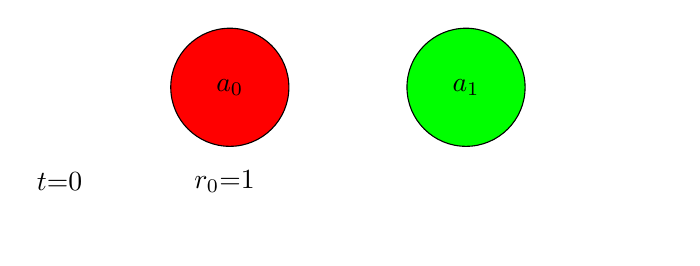
\begin{tikzpicture}
\node[draw,circle, minimum size=1.5cm, inner sep=2pt, black, fill=red] at (2,0) {$a_0$};
\node[draw,circle,minimum size=1.5cm,inner sep=0pt,black,fill=green] at (5,0) {$a_1$};
%\node[draw,circle,minimum size=1.5cm,inner sep=0pt,black,fill=yellow] at (8,0) {$a_2$};
\node[text width=3cm] at (1.05,-1.2) 
    {$t$=0};
\node[text width=3cm] at (3.05,-1.2) 
    {$r_0$=1};
\node[text width=3cm] at (6.0,-1.8) 
    {};
\end{tikzpicture}

\end{center}
\end{frame}

\begin{frame}{Example}
\begin{center}
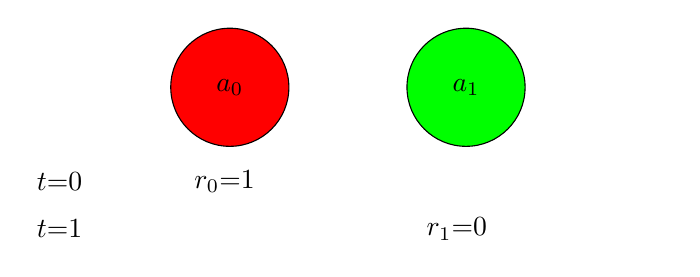
\begin{tikzpicture}
\node[draw,circle, minimum size=1.5cm, inner sep=2pt, black, fill=red] at (2,0) {$a_0$};
\node[draw,circle,minimum size=1.5cm,inner sep=0pt,black,fill=green] at (5,0) {$a_1$};
%\node[draw,circle,minimum size=1.5cm,inner sep=0pt,black,fill=yellow] at (8,0) {$a_2$};
\node[text width=3cm] at (1.05,-1.2) 
    {$t$=0};
\node[text width=3cm] at (3.05,-1.2) 
    {$r_0$=1};
\node[text width=3cm] at (1.05,-1.8) 
    {$t$=1};
\node[text width=3cm] at (6.0,-1.8) 
    {$r_1$=0};
\end{tikzpicture}

\end{center}
\end{frame}

\begin{frame}{Example}
\begin{center}
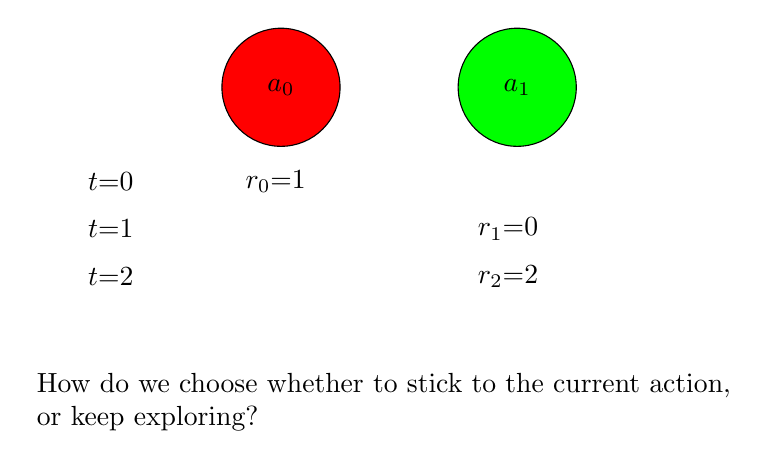
\begin{tikzpicture}
\node[draw,circle, minimum size=1.5cm, inner sep=2pt, black, fill=red] at (2,0) {$a_0$};
\node[draw,circle,minimum size=1.5cm,inner sep=0pt,black,fill=green] at (5,0) {$a_1$};
%\node[draw,circle,minimum size=1.5cm,inner sep=0pt,black,fill=yellow] at (8,0) {$a_2$};
\node[text width=3cm] at (1.05,-1.2) 
    {$t$=0};
\node[text width=3cm] at (3.05,-1.2) 
    {$r_0$=1};
\node[text width=3cm] at (1.05,-1.8) 
    {$t$=1};
\node[text width=3cm] at (6.0,-1.8) 
    {$r_1$=0};
\node[text width=3cm] at (6.0,-2.4) 
    {$r_2$=2};
\node[text width=3cm] at (1.05,-2.4) 
    {$t$=2};
\node[text width=9cm] at (3.4,-4) 
    {How do we choose whether to stick to the current action, or keep exploring?};  
\end{tikzpicture}

\end{center}
\end{frame}

\begin{frame}{Exploration-Exploitation Trade-off}
\section{Exploration-Exploitation Trade-off}

To maximize its reward in this environment, our agent must learn what the best action to take is.

\vspace{2mm}
	
\begin{itemize}
    \item \textcolor{RoyalBlue}{Exploration} allows to gain knowledge of its actions, useful for the \textbf{long-term}
   \item \textcolor{RoyalBlue}{Exploitation} allows to use the current knowledge of the actions to get an \textbf{instantaneous benefit}
\end{itemize}

\end{frame}





\begin{frame}{Action-Value Methods}
\section{Action-Value Methods}

The \textcolor{RoyalBlue}{action value} for action a is the reward we expect to receive by taking that action:

\begin{align*}
	Q^{*}(a) \doteq \mathds{E}[R_t|a_t = a]
\end{align*}

The goal is to find the \textcolor{RoyalBlue}{optimal value}, by maximizing the expected cumulative reward:

\begin{align*}
    a_{*} =\underset{a}{\argmax}\:\mathds{E}[R_t|a_t = a]
\end{align*}

\textcolor{RoyalBlue}{Regret} of an action $a$:
\begin{align*}
    \Delta_a = a_{*} - Q(a)
\end{align*}

\end{frame}


\begin{frame}{Action-Value Methods}

In Reinforcement Learning we do not know which actions have the best value: we need to learn it.

\vspace{2mm}

\begin{block}{Action Value Estimate}		
We denote the estimated value of action $a$ at time step $t$ as $Q_t(a)$.
\end{block}

\vspace{2mm}

We can use action value estimates to learn a policy.

\end{frame}

\begin{frame}{Sample-average Method}

The simplest estimate is given by the average of the sampled rewards:

\begin{align*}
	Q_t(a) &\doteq \frac{\text{sum of rewards when $a$ taken prior to $t$}}{\text{number of times $a$ taken prior to $t$} }\\
	   & = \frac{\sum_{i=0}^{T} R_i \cdot \mathds I(A_i = a)}{\sum_{i=0}^{T} \mathds I(A_i = a)}
\end{align*}

$\mathds I$ is the \textcolor{RoyalBlue}{indicator function}: $\mathds I(True) = 1$, and $\mathds I(False) = 0$.
 
\end{frame}


\begin{frame}{Incremental Update}

The sample-average method can be computed incrementally:

\begin{align*}
	Q_{t+1}(a) &= \frac{1}{t+1} \sum_{i=0}^{t+1} R_i \\
	           &= \frac{1}{t} \bigg[ R_t + (t-1)\frac{1}{t-1}\sum_{i=0}^{t-1} R_i \bigg]\\
	           &= \frac{1}{t} \bigg[ R_t + (t-1) Q_t(a) \bigg ]\\
	           &= Q_t(a) + \frac{1}{t}  \bigg[ R_t - Q_t(a)  \bigg ]
\end{align*}


\end{frame}


\begin{frame}{Incremental Update}

\begin{align*}
	Q_{t+1}(a) = Q_t(a) + \alpha_t ( R_t - Q_t(a)) \hspace{4mm} \text{where} \hspace{4mm} \alpha_t = \frac{1}{t}
\end{align*}


\begin{block}{Update Rule}		
\begin{align*}
    NewEstimate \leftarrow OldEstimate + StepSize [Target - OldEstimate]
\end{align*}\end{block}


\vspace{4mm}

Later we will consider other possible step sizes $\alpha_t$.

\end{frame}

\begin{frame}{Action Selection: greedy}

Action-value estimates can be used to select actions. 

\vspace{4mm}

We can exploit the current knowledge by selecting the \textcolor{RoyalBlue}{greedy} action, which is the action with the highest estimated value:


\begin{align*}
A_{t} =\underset{a \in \mathcal{A}}{\argmax} \; Q_t(a)
\end{align*}

\textcolor{Maroon}{Downside}: we can get stuck taking a \textcolor{RoyalBlue}{suboptimal action} forever, because we are not exploring better opportunities.

\end{frame}


\begin{frame}{Action Selection: $\epsilon-$greedy}



\begin{itemize}
    \item Behave \textcolor{RoyalBlue}{greedily} with probability $1-\epsilon$
    \item Take a \textcolor{RoyalBlue}{random action} with probability $\epsilon$
\end{itemize}

\vspace{2mm}

Where $\epsilon$ is a small, positive number $0 < \epsilon < 1$.

\begin{align*}
 \pi_t(a) =
    \begin{cases}
      (1-\epsilon) + \epsilon/|\mathcal{A}| \hspace{2mm} \text{if} \hspace{2mm} a=\underset{a \in \mathcal{A}}{\argmax} \; Q_t(a)\\
       \epsilon/|\mathcal{A}|  \hspace{18mm} \text{otherwise}
    \end{cases}       
\end{align*}

%\begin{align*}
% A_t =
%    \begin{cases}
%      \underset{a}{\argmax} Q_t(a)  & \text{with probability $\epsilon$}\\
%      \text{random action} & \text{with probability $1-\epsilon$}
%    \end{cases}       
%\end{align*}

\end{frame}




\begin{frame}{Optimistic Initial Values}

All the methods discussed up to now depend on the \textcolor{RoyalBlue}{initial values} of the action estimates,  $Q_0(a) \; | a \in \matchcal{A}$.

\vspace{5mm}

Optimistic initial values can be used to \textcolor{RoyalBlue}{encourage early exploration}:

\vspace{1mm}
\begin{itemize}
    \item For any starting action taken by the agent, the reward is smaller than the starting estimates
    \item The agent, disappointed, switches to other actions
    \item Actions are tried several times before the value estimates converge
\end{itemize}
\end{frame}

\begin{frame}{Uncertainty in Action Values Estimates}

If we could explicit the \textcolor{RoyalBlue}{uncertainty} of our action-values estimates, we could select actions in a better way.

\vspace{5mm}

\begin{tikzpicture}
\node[text width=3cm] at (5.2,0.5) {$Q(a)$};  
\draw (0,0) -- (2.5,0) node {[} --  (5.5,0) node {]} -- (8,0);
\draw [red] (4,-0.25) -- (4,0.25);
\end{tikzpicture}

\vspace{5mm}

Select actions by leveraging their uncertainty: if we are uncertain about the value of an action, we \textcolor{RoyalBlue}{optimistically assume that it is good}.

\end{frame}


\begin{frame}{Optimism in the Face of Uncertainty}


%\vspace{3mm}

\begin{tikzpicture}
\node[text width=3cm] at (6.2,0.5) {$Q_0$};  
\draw (0,0) -- (2.5,0) node {[} --  (7,0) node {]} -- (8,0);
\draw [red] (4.8,-0.25) -- (4.8,0.25);
\draw [stealth-, red](8.5,0) -- (9.5,0);

\node[text width=3cm] at (4.1,-0.9) {$Q_1$};  
\draw (0,-1.5) -- (1.5,-1.5) node {[} --  (4,-1.5) node {]} -- (8,-1.5);
\draw [red] (2.8,-1.2) -- (2.8,-1.8);

\node[text width=3cm] at (6.8,-2.5) {$Q_2$};  
\draw (0,-3) -- (5,-3) node {[} --  (6,-3) node {]} -- (8,-3);
\draw [red] (5.5,-2.75) -- (5.5,-3.25);

\draw [dashed] (7,0.7) -- (7,-3.8);
\end{tikzpicture}

\end{frame}


\begin{frame}{Optimism in the Face of Uncertainty}

%How can we take actions leveraging their uncertainty?

%\vspace{2mm}

\begin{tikzpicture}
\node[text width=3cm] at (5.8,0.6) {$Q_0$};  
\draw (0,0) -- (4.,0) node {[} --  (5.,0) node {]} -- (8,0);
\draw [red] (4.5,-0.25) -- (4.5,0.25);

\node[text width=3cm] at (4.1,-0.9) {$Q_1$};  
\draw (0,-1.5) -- (1.5,-1.5) node {[} --  (4,-1.5) node {]} -- (8,-1.5);
\draw [red] (2.8,-1.2) -- (2.8,-1.8);

\node[text width=3cm] at (6.8,-2.5) {$Q_2$};  
\draw (0,-3) -- (5,-3) node {[} --  (6,-3) node {]} -- (8,-3);
\draw [red] (5.5,-2.75) -- (5.5,-3.25);

\draw [dashed] (6,0.7) -- (6,-3.8);
\end{tikzpicture}


\end{frame}


\begin{frame}{Upper-Confidence Bound (UCB)}

We want to estimate an upper confidence bound for every action value:

\begin{align*}
q_t \leq Q_{t}(a) + U_t(a)
\end{align*}

And select \textcolor{RoyalBlue}{greedily} the action maximizing the UCB:

\begin{align*}
a_t \doteq \argmax_{a \in \mathcal{A}} Q_t(a) + U_t(a)
\end{align*}


\end{frame}


%\begin{frame}{Upper Confidence Bound (UCB)}
%We want to select an action $a$ if:
%\begin{itemize}
%    \item the action value estimate $Q_t(a)$ is large
%    \item the uncertainty $U_t(a)$ is large
%\end{itemize}
%\end{frame}


\begin{frame}{Upper-Confidence Bound (UCB)}
\begin{align*}
a_t \doteq \argmax_{a \in \mathcal{A}} \bigg [ Q_t(a) + c \sqrt{\frac{ln(t)}{N_a(t)}} \bigg ]
\end{align*}

\hspace{3mm}

\begin{itemize}
    \item Each time we select $a$, $N_a(t)$ is increased and therefore the uncertainty is reduced
    \item Each time we select $a^{\prime} \neq a$, $t$ increases but $N_a(t)$ does not, therefore the uncertainty increases
\end{itemize}

\hspace{2mm}

The parameter $c > 0$ regulates the amount of exploration.

\end{frame}


\begin{frame}{Action Preferences}
\section{Action Preferences}

All methods described until now rely on the estimate of action values to learn a policy.
Another approach relies on learning a \textcolor{RoyalBlue}{preference for each action}, $H_t(a)$.

\vspace{1mm}

\begin{itemize}
    \item The larger the preference, the more probably a certain action should be selected
    \item The preference has no meaning in terms of reward
\end{itemize}

\vspace{1mm}

\begin{block}{Boltzmann distribution}
From the action preferences, we can define a policy using the \textcolor{RoyalBlue}{Softmax or Boltzmann} distribution:
\begin{align*}
    \pi(a) = \frac{e^{H_t(a)}}{\sum_{k=0}^{N} e^{H_t(k)}}
    \end{align*}
\end{block}

\textcolor{Maroon}{Note}: You will use this distribution in deep learning when it comes to multi-class classification problems!

\end{frame}


%\begin{frame}{Gradient Ascent}

%We will optimize the policy by optimizing the preferences. Preferences can be considered as \textcolor{RoyalBlue}{policy parameters}:

%\begin{align*}
%    \pi_t(a) = \pi_t(a,\theta_{t})
%\end{align*}

%Gradient ascent: 

%\begin{align*}
%    \theta_{t+1} = \theta_t + \alpha \nabla_{\theta} \matchcal{E}[R_t | \pi_{\theta}_t]
%\end{align*}

%\end{frame}

\begin{frame}{Action Preferences}

If at time step $t$ we choose action $a^{\prime}$, we can update the action preferences as:

\begin{align*}
H_{t+1}(a^{\prime}) \doteq H_t(a^{\prime}) + \alpha \: r_t (1 - \pi_t(a^{\prime}))\\
H_{t+1}(a) \doteq H_t(a) + \alpha \: r_t \: \pi_t(a^{\prime}) \; \text{ if } \; a \neq a^{\prime}
\end{align*}

\vspace{2mm}

Where the formula above is based on the idea of stochastic gradient ascent.


\end{frame}

\begin{frame}{Associative Search: Contextual Bandits}

Until now, we considered contexts where the agent has to learn how to behave in a \textcolor{Maroon}{single situation}.
However, the general problem of Reinforcement Learning deals with learning how to behave in a number of \textcolor{RoyalBlue}{different situations}.

\end{frame}

\begin{frame}{Associative Search: Contextual Bandits}

Simple way to extend bandits:

\vspace{2mm}

\begin{itemize}
    \item You face $N$ different Multi-Armed bandit problems%, where you are given some kind of information in order to distinguish among those
    \item This is an \textcolor{RoyalBlue}{associative task}: $\pi: \mathcal{S}\rightarrow \mathcal{A}$
    \item Similar to the full Reinforcement Learning problem as they involve \textcolor{RoyalBlue}{learning a policy}, but like the k-armed bandit problem in that each action affects only the \textcolor{RoyalBlue}{immediate reward}.
\end{itemize}

\end{frame}


%\begin{frame}{Bayesian Bandits}
%\section{Bayesian Bandits}
%The Bayesian approach can model the \textcolor{RoyalBlue}{uncertainty} over the expected value of each action: $p(q(a) \; | \; \theta_t)$
%\begin{itemize}
%    \item $\theta_t$ are the parameters of our distribution.
%    \item We can use the distribution to drive exploration.
%\end{itemize}
%\end{frame}


%\begin{frame}{Bayesian Bandits}
%\begin{itemize}
%    \item Consider a Bandit with \textcolor{RoyalBlue}{Bernoulli distributions} on each arm: rewards can be 0 or 1.
%    \begin{align*}P(r_t=1) = p,  \hspace{3.5mm}  P(r_t=0) = 1-p\end{align*}
%    \item We want to pick the action which gives 1 more often
%\end{itemize}
%\end{frame}


\begin{frame}{Final Slide!}
	\begin{takeaway}{Lecture Takeaway}
		\begin{enumerate}
		    \item Multi-Armed bandit is a simplified setting with a single state
		    \item To learn a policy we need to balance Exploration and Exploitation
			\item We can learn the policy by leveraging action-values estimates $Q(a)$
			\item Or by leveraging action preferences $H(a)$
		\end{enumerate}
	\end{takeaway}
\end{frame}

\end{document}
